 \documentclass[12pt]{article}
 \usepackage{makecell}
 \usepackage{float}
\usepackage{graphicx}
\usepackage{booktabs}
\usepackage[margin=1in]{geometry}
\usepackage{fancyhdr}
\pagestyle{fancy}
\usepackage{extarrows}
\usepackage{breqn}

\newcommand{\N}{\mathbb{N}}
\newcommand{\Z}{\mathbb{Z}}
\newcommand{\trans}{^{\mathrm T}}
\DeclareMathOperator{\tr}{tr}
\DeclareMathOperator{\rank}{rank}
\DeclareMathOperator{\Span}{span}
\DeclareMathOperator{\row}{row}
\DeclareMathOperator{\col}{col}
\DeclareMathOperator{\range}{range}
\DeclareMathOperator{\Null}{Null}
\DeclareMathOperator{\Proj}{Proj}
\newcommand{\diff}{\,\mathrm{d}}
\DeclareMathOperator{\trace}{trace}
\newcommand{\Her}{^{\mathrm H}}
\DeclareMathOperator{\diag}{diag}
\usepackage{amssymb}
\usepackage[table]{xcolor}
\usepackage{bm}
\usepackage{array}
\usepackage{mathtools}
\usepackage[english]{babel}
\usepackage{natbib}
\usepackage{url}
\usepackage[utf8x]{inputenc}
\usepackage{amsmath}
\usepackage{graphicx}
\graphicspath{{images/}}
\usepackage{parskip}
\usepackage{fancyhdr}
\usepackage{vmargin}
\usepackage[font={bf, footnotesize}, textfont=md]{caption}
\makeatletter 
    \newcommand\fcaption{\def\@captype{table}\caption}
\makeatother
\setmarginsrb{3 cm}{2.5 cm}{3 cm}{2.5 cm}{1 cm}{1.5 cm}{1 cm}{1.5 cm}

\title{Lab Report for Rotational Inertia}                             % Title
\author{Jie Wang}                               % Author
\date{\today}                                           % Date

\makeatletter
\let\thetitle\@title
\let\theauthor\@author
\let\thedate\@date
\makeatother

\pagestyle{fancy}
\fancyhf{}
\rhead{\theauthor}
\lhead{\thetitle}
\cfoot{\thepage}

\begin{document}

%%%%%%%%%%%%%%%%%%%%%%%%%%%%%%%%%%%%%%%%%%%%%%%%%%%%%%%%%%%%%%%%%%%%%%%%%%%%%%%%%%%%%%%%%

\begin{titlepage}
    \centering
    \vspace*{0.5 cm}
    
\includegraphics[scale = 0.75,width=6cm]{CUHK}\\[1.0 cm]   % University Logo
    \textsc{\large The Chinese University of Hong Kong, Shenzhen}\\[2.0 cm]   % University Name
    \textsc{\Large PHY 1002}\\[0.5 cm]               % Course Code
    \textsc{\large Physics Laboratory}\\[0.5 cm]               % Course Name
    \rule{\linewidth}{0.2 mm} \\[0.4 cm]
    { \huge \bfseries \thetitle}\\
    \rule{\linewidth}{0.2 mm} \\[1.5 cm]
    
    \begin{minipage}{0.4\textwidth}
        \begin{flushleft} \large
            \emph{Author:}\\
            \theauthor
            \end{flushleft}
            \end{minipage}~
            \begin{minipage}{0.4\textwidth}
            \begin{flushright} \large
            \emph{Student Number:} \\
            116010214                                   % Your Student Number
        \end{flushright}
    \end{minipage}\\[2 cm]
    
    {\large \thedate}\\[2 cm]
 
    \vfill
    
\end{titlepage}

%%%%%%%%%%%%%%%%%%%%%%%%%%%%%%%%%%%%%%%%%%%%%%%%%%%%%%%%%%%%%%%%%%%%%%%%%%%%%%%%%%%%%%%%%
%%%%%%%%%%%%%%%%%%%%%%%%%%%%%%%%%%%%%%%%%%%%%%%%%%%%%%%%%%%%%%%%%%%%%%%%%%%%%%%%%%%%%%%%%

\tableofcontents
\pagebreak

%%%%%%%%%%%%%%%%%%%%%%%%%%%%%%%%%%%%%%%%%%%%%%%%%%%%%%%%%%%%%%%%%%%%%%%%%%%%%%%%%%%%%%%%%

\rmfamily
\section{Experiment 1 Physical Pendulum – Period}
\subsection{Objective:}
This experiment is designed to \emph{explore} the relationship between the \emph{period of a physical pendulum} (a \textbf{uniform bar}) and \emph{the distance from the pivot point to the center of mass}. During this process, we will study \emph{how the period changes as pivot is moved from the first hole of the bar to the center.} Then we measure the distance from the \emph{piovt point} to the \emph{center of mass} that produces the \emph{minimum} period of oscillation. Comparing it to the theoretical value, if the error is acceptable, the validity of this experiment is confirmed.

\subsection{Theory}
Recall that the momentum of inertia of a \emph{long rod} about its center of mass is:
\begin{equation}
I_{\text{c}} = \frac{1}{12}ML^2
\label{Eq._3}
\end{equation}
where $M$ is its mass, and $L$ is the overall length of rod.\\
A more precise physical model of the momentum of inertia for the uniform bar as a \emph{rectangle-type} rod is:
\[
I_{\text{c}} = \frac{1}{12}M(a^2+b^2)
\]
where $a$ is its length and $b$ is its thickness.\\ However, in this case $a>>b$, ($\left(\frac{b}{a}\right)^2<0.003$) so $I_{\text{c}} = \frac{1}{12}ML^2$ could be used as a very good approximation.(error is only $0.3\%$.)\\
The period of a physical pendulum depends on its momentum of inertia $I_{\text{pivot}}$, its mass $M$ and the distance from the pivot point to the center of mass $L_{\text{c}}$:
\begin{equation}
T=2\pi\sqrt{\frac{I_{\text{pivot}}}{MgL_{\text{c}}}}\label{Eq._1}
\end{equation}
And the \emph{parallel axis theorem} enables us to write the momentum of inertia of the bar about a \emph{pivot point} as:
\begin{equation}\label{Eq._2}
I_{\text{pivot}} = I_{\text{c}}+ML_{\text{c}}^2
\end{equation}
Combining the Eq.(\ref{Eq._3}), Eq.(\ref{Eq._1}) and Eq.(\ref{Eq._2}), we derive the period of the pendulum:
\begin{equation}
T=2\pi\sqrt{\frac{\frac{1}{12}L^2+L_{\text{c}}^2}{gL_{\text{c}}}}\label{Eq._4}
\end{equation}
Setting the derivative equal to zero and solve for $L_{\text{c}}$, we obtain the theoratical value which produces the \emph{minimum} period oscillation for the bar:
\begin{equation}
L_{\text{c}}^0=\frac{1}{\sqrt{12}}L.\label{Eq._5}
\end{equation}




\subsection{Method:}
\begin{enumerate}
\item
We completed the full setup. (Refer to \textit{Capstone Physical Pendulum -- Period manual} for detail reading)
\item
We gently stated the pendulum bar swing with a \emph{small amplitude} (about 20 degrees total)
\item
Then we clicked on ``\emph{Record}'' on Capstone to begin recording data. After about $25$ seconds, click ``\emph{STOP}'' to stop recording data. Data would appear in the graph of \emph{angular position} versus \emph{time}. From the graph we determined and recorded the \emph{period} of this oscillation.
\item
Then we moved the mounting screw to the next hole (4cm from the center hole) and repeated step $\bm 2-\bm3$. Then we repeated the process for the holes that are 6cm, 8cm, 10cm, 12cm and 14cm from the center hole.
\end{enumerate}
\subsection{Raw Data:}
The table(\ref{Data for period versus length: Collected from Capstone}) below shows typical data for the length from the \emph{pivot point} to the \emph{center of mass} of an oscillating pendulum bar and the corresponding \emph{period} of oscillation for each length:
\begin{center}
\begin{tabular}{|p{3cm}<{\centering}|p{5cm}<{\centering}|}
\hline
Length			&			Period\\
(cm)	 $(\pm0.05\text{cm})$			&			(sec)$(\pm3.16\times10^{-4}\text{s})$	\\
\hline
2.0				&			1.195	\\
\hline
4.0				&			0.928	\\
\hline
6.0				&			0.839	\\
\hline
8.0				&			0.823	\\
\hline
10.0				&			0.824	\\
\hline
12.0				&			0.850	\\
\hline
14.0				&			0.878\\
\hline
\end{tabular}
\fcaption{Data for period versus length: Collected from Capstone}\label{Data for period versus length: Collected from Capstone}
\end{center}
\begin{itemize}
\item
\textbf{Error Explanation: }The error for the length $\delta_{L_c}$ is due to the \emph{systematic error}, thus $\delta_{L_c}=5\times10^{-4}$m. And the error for the period is due to the \emph{propagation error}:
\begin{itemize}
\item
Since $T=2\pi\sqrt{\frac{\frac{1}{12}L^2+L_{\text{c}}^2}{gL_{\text{c}}}}$, its error could be computed as:
\begin{align*}
\delta T&=\sqrt{\left(\frac{\partial T}{\partial L_{c}}\right)^2(\delta_{L_c})^2}\\
&=\left|\frac{\partial T}{\partial L_{c}}\right|\cdot(\delta_{L_c})\\
&=\pi\left(\frac{\frac{1}{12}L^2+L_c^2}{gL_c}\right)^{-1/2}\times\frac{\left|(\frac{1}{12}L^2+L_c^2)-(2L_c)^2\right|}{(gL_c)^2}\cdot(\delta_{L_c})\\
&\le
\pi\left(\frac{\frac{1}{12}(0.28\text{m})^2+(0.14\text{m})^2}{9.8\text{m/}s^2\cdot (0.14\text{m})}\right)^{-1/2}\times\frac{\left|(\frac{1}{12}(0.28\text{m})^2+(0.14\text{m})^2)-(0.28\text{m})^2\right|}{(9.8\text{m/}s^2\cdot (0.14\text{m}))^2}\cdot(\delta_{L_c})\\
&=0.6320\times5\times10^{-4}\text{m}\\&=3.16\times10^{-4}\text{s}.
\end{align*}
\end{itemize}
\end{itemize}
\subsection{Data Analysis}
We use the data from Table(\ref{Data for period versus length: Collected from Capstone}) to draw the \emph{period} versus \emph{length} curve. (As Figure(\ref{F_4_1}) shown) As the length from the \emph{pivot point} to the \emph{center of mass} increasing, the period decreased and then increased.
\begin{figure}[H]
\centering
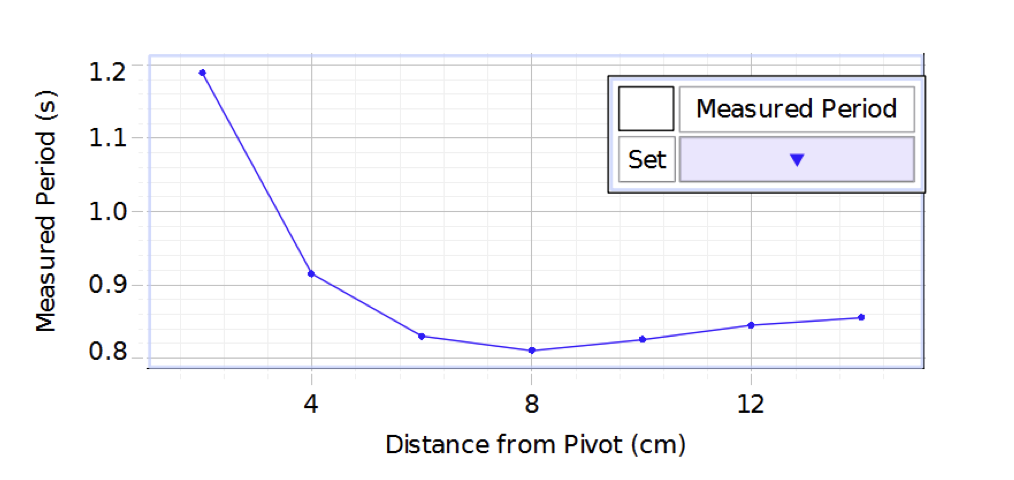
\includegraphics[width=10cm]{f_4_1}
\caption{Experimental Period ($T$) versus Length ($L_{\text{c}}$) graph: data from Table(1)}
\label{F_4_1}
\end{figure}
The theoretical value for the period is obtained from Eq.(\ref{Eq._4}), where $L=28$cm, $g=9.8m/s^2$. Thus we could plot the \emph{theoretical} period versus length $L_{\text{c}}$ graph:
\begin{figure}[H]
\centering
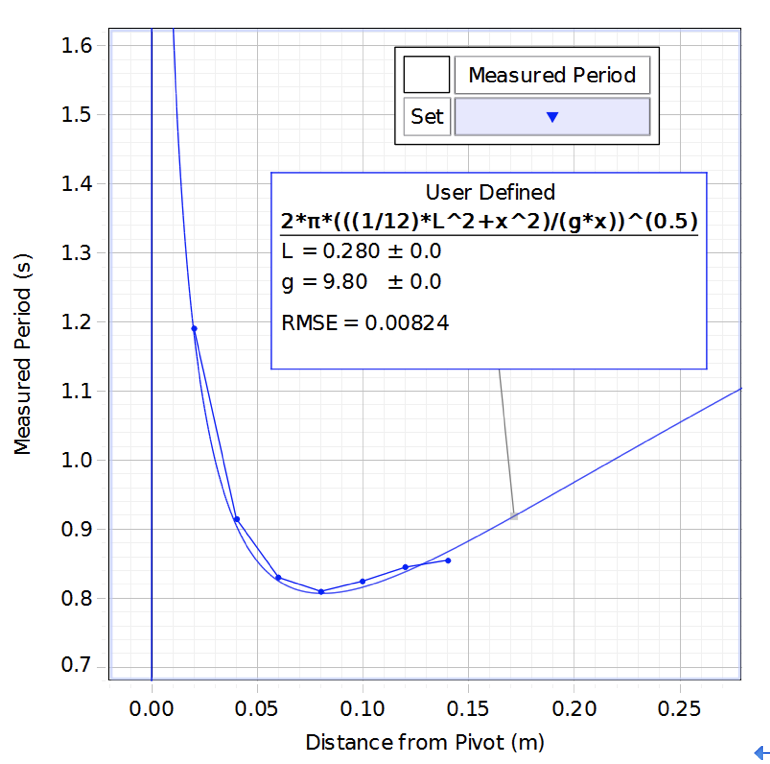
\includegraphics[width=8cm]{f_4_2}
\caption{Theoretical Period ($T$) versus Length ($L_{\text{c}}$) graph}
\label{Theoretical}
\end{figure}
We observe that there is an error between the experimental and theoretical value for the \emph{period} in Figure(\ref{Theoretical}). In order to reduce the error, we could remove several points from Table(\ref{Data for period versus length: Collected from Capstone}). Finally, we find the experimental period at length $6$cm, $8$cm, $10$cm fit the theoretical curve better:
\begin{figure}[H]
\centering
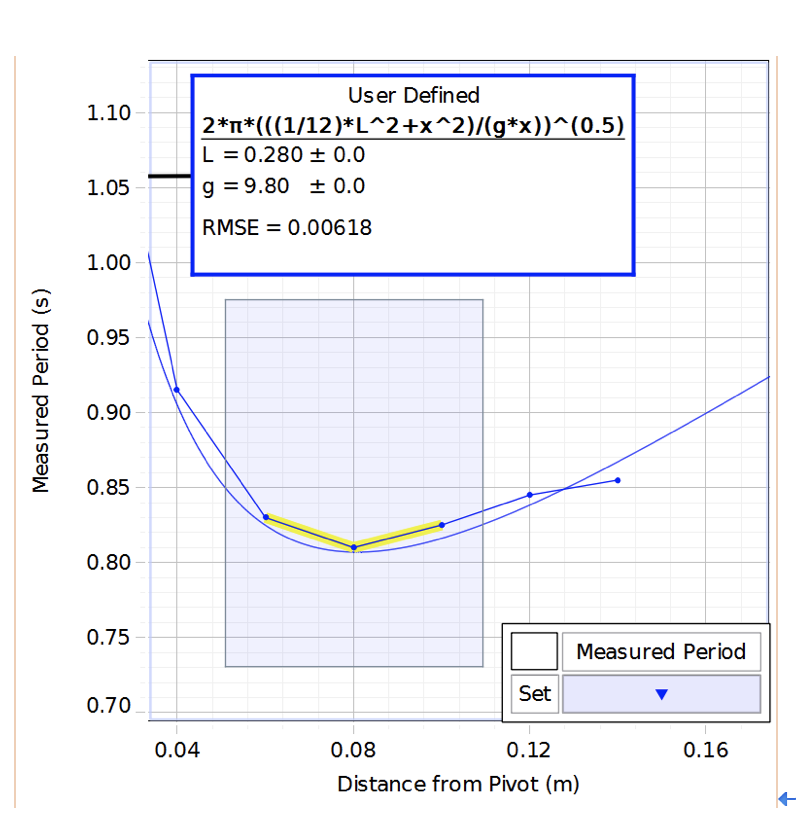
\includegraphics[width=8cm]{f_4_3}
\caption{Improved experimental results by ignoring several data}
\label{Theoretical}
\end{figure}
Finally, we unlock the value of length of pendulum and gravity and updated the fitted curve: (Shown in Figure(\ref{Fitted curves}))
\begin{figure}[H]
\centering
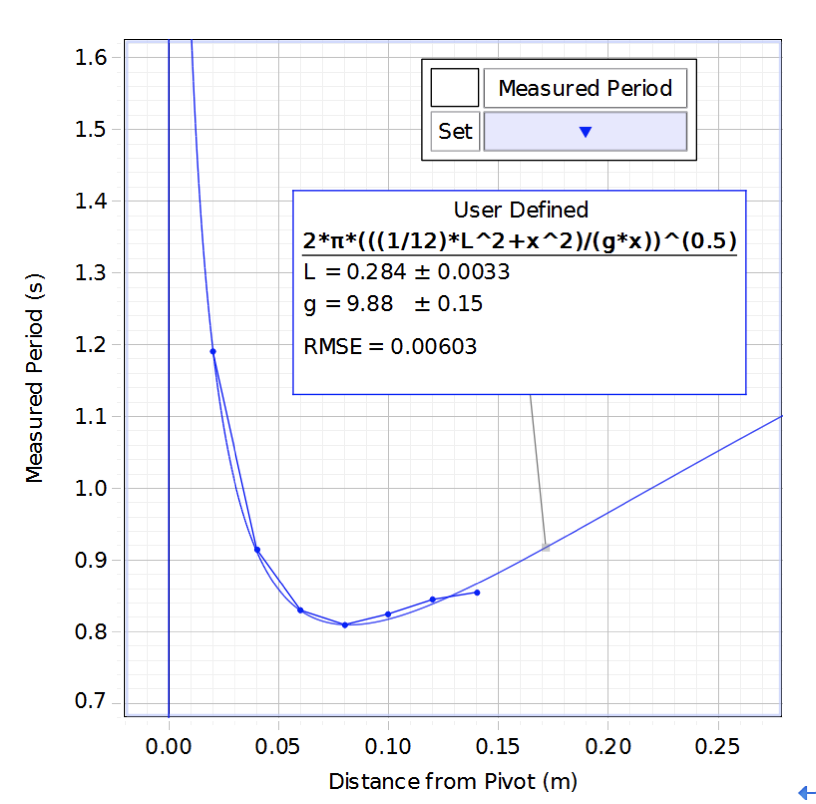
\includegraphics[width=8cm]{f_4_4}
\caption{Fitted curves for the data from Table(\ref{Data for period versus length: Collected from Capstone})}
\label{Fitted curves}
\end{figure}
Thus we find the updated parameter value for the length $L$ and the gravity $g$:
\[
L_{Fitted} = 0.284\pm0.0033\text{m}.
\]
\[
g_{Fitted} = 9.88\pm0.15\text{m/}s^2.
\]
\subsubsection{Difference}
In Figure(\ref{Fitted curves}), we found the parameters $L$ and $g$ are very close to the actual value. The differnce for $L$ is given by:
\begin{align*}
\text{Difference}&=\frac{L_{\text{Fitted}}-L_{\text{Actual Value}}}{L_{\text{Actual Value}}}\times100\%\\
&=\frac{0.284\text{m}-0.280\text{m}}{0.280\text{m}}\times100\%\\
&=1.43\%
\end{align*}
The difference for $g$ is given by:
\begin{align*}
\text{Difference}&=\frac{g_{\text{Fitted}}-g_{\text{Actual Value}}}{g_{\text{Actual Value}}}\times100\%\\
&=\frac{9.88\text{m/}s^2-9.80\text{m/}s^2}{9.80\text{m/}s^2}\times100\%\\
&=0.82\%
\end{align*}
From Table(\ref{Data for period versus length: Collected from Capstone}), we find the measured value for length that gives minimum period is $L_{\text{measured}}=8.0\pm0.05$cm. And due to Eq.(\ref{Eq._5}), the theoretical value for length that gives minimum period is:
\[
L_{\text{c}}^0=\frac{1}{\sqrt{12}}\times (28.0\pm0.05)\text{cm}=8.1\pm0.01\text{cm}
\]
Hence the percent difference between the theoretical and experimental length that produces minimum period is:
\begin{align*}
\text{Difference}&=\frac{L_{\text{measured}}-L_{\text{c}}^0}{L_{\text{c}}^0}\times100\%\\
&=\frac{8.0\text{cm}-8.1\text{cm}}{8.1\text{cm}}\times100\%\\
&=1.23\%
\end{align*}





\section{Experiment 2 Rotational Inertia Based on Period of Oscillation}
\subsection{Objective:}
During this experiment, 
\begin{itemize}
\item
Firstly, we measured the \emph{mass}, the \emph{dimensions} and the distance from pivot point to its center of mass to derive the \emph{theoretical value of inertia of a physical pendulum}. (By Rotational Inertia Equations)
\item
Then we measured the \emph{period of oscillation of a physical pendulum} to compute the \emph{momentum of inertia indirectly}.
\item
And we also calculated the \emph{rotational inertia} of a \textbf{irregular shape disk} about the center of mass based on \emph{angular acceleration}.
\end{itemize}
We compare the results from these different methods, if the error is acceptable, we conclude the validity of this experient.
\subsection{Theory:}
\subsubsection{Method 1:}
The theoretical momentum of inertia about its center of mass could be derived from its mass, the dimensions and the distance from pivot point to its center of mass. We have different kinds of disks shown in Figure(\ref{Different kinds of disks}):
\begin{figure}[H]
\centering
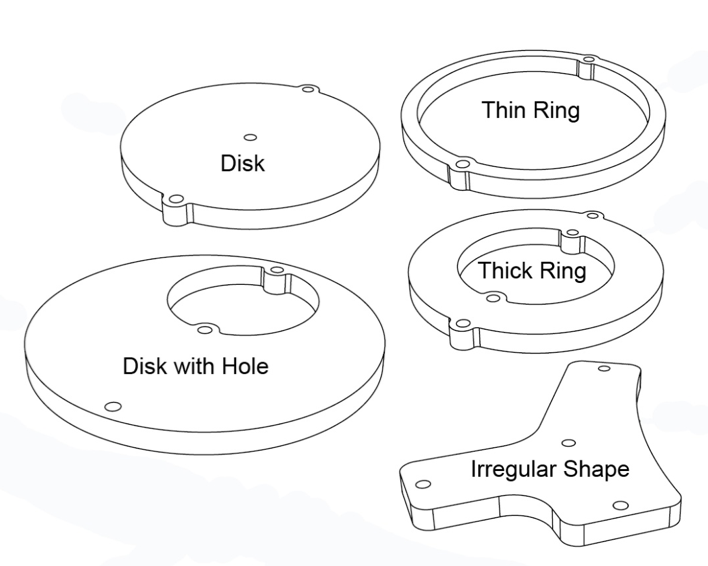
\includegraphics[width=8cm]{f_4_5}
\caption{Different kinds of disks}
\label{Different kinds of disks}
\end{figure}
For the first disk, its momentum of inertia about its center of mass is given by:
\begin{equation}
I=\frac{1}{2}MR^2\label{Eq._6}
\end{equation}
where $M$ denotes its mass and $R$ denotes its radius.\\
For the thick ring, its momentum of inertia about its center of mass is given by:
\begin{equation}
I=\frac{1}{2}M(R_1^2+R_2^2)\label{Eq._7}
\end{equation}
where $M$ denotes its mass, $R_1$ denotes its  outer radius, $R_2$ denotes its inner radius.\\
For the thin ring, its momentum of inertia about its center of mass is given by:
\begin{equation}
I=MR^2\label{Eq._8}
\end{equation}
where $M$ denotes its mass and $R$ denotes its radius.\\
For a disk of radius $R$ with a hole of radius $r$, we pivoted at the outer edge of the hole:
\begin{align*}
I&=I_{\text{disk}}-I_{\text{hole}}=\left(\frac{1}{2}M_{\text{disk}}R^2+M_{\text{disk}}L_c^2\right)
-
\left(\frac{1}{2}M_{\text{hole}}r^2+M_{\text{hole}}r^2\right)\\
&=\frac{1}{2}M_{\text{disk}}R^2+M_{\text{disk}}L_c^2-\frac{3}{2}M_{\text{hole}}r^2
\end{align*}
where $R$ denotes the radius of the disk, $r$ denotes the radius of the hole, $M$ denotes the mass of the disk, $L_c$ denotes the distance from the pivot to the center of mass. Assuming the mass is uniformly distributed on the disk, then we derive:
\[
M_{\text{disk}}=\sigma A_{\text{disk}}=\frac{M}{(\pi R^2-\pi r^2)}(\pi R^2)=M\left(\frac{R^2}{R^2-r^2}\right),
\]
\[
M_{\text{hole}}=\sigma A_{\text{hole}}=\frac{M}{(\pi R^2-\pi r^2)}(\pi r^2)=M\left(\frac{r^2}{R^2-r^2}\right).
\]
Finally, the momentum of inertia for a disk with a hole is given by:
\begin{align}
I&=\frac{1}{2}M\left(\frac{R^2}{R^2-r^2}\right)
+M\left(\frac{R^2}{R^2-r^2}\right)L_c^2-\frac{3}{2}M\left(\frac{r^2}{R^2-r^2}\right)r^2\\
&=\frac{1}{2}M\left(\frac{R^4-3r^4+2R^2L_c^2}{R^2-r^2}\right)
\label{Eq._10}
\end{align}
We \textbf{cannot} compute the theoretical momentum of inertia for irregular shape disk in this way. 
\subsubsection{Method 2:}
We could compute the rotational inertia indirectly. By Eq.(\ref{Eq._1}) and Eq.(\ref{Eq._2}), the \emph{period of oscillation} $T$ of a physical pendulum, depends on the \emph{momentum of inertia anout the center of mass} $I_{\text{c}}$, the mass $M$, the \emph{distance} from the pivot point to the center of mass $L_{\text{c}}$:
\[
T=2\pi\sqrt{\frac{I_{\text{c}}+ML_{c}^2}{MgL_{c}}}
\]
Conversely, the momentum of inertia about its center of mass could be found as follows:
\begin{equation}
I_{\text{c}}=\frac{T^2MgL_{c}}{4\pi^2}-ML_{c}^2.
\label{Method_1}
\end{equation}
\subsubsection{Method 3:}
We use another way to compute the inertia of \textbf{irregular shape of disk}. We apply the formula
\[
\tau = I\alpha\implies
I=\frac{\tau}{\alpha}
\]
where $\tau$ is the torque caused by the weight hanging from the string which is wrapped around the large step of the 3-steo pulley of the apparatus. $\alpha$ denotes the angular acceleration. And we also obtain:
\[
\tau = rF
\]
where $r$ is the radius of the pulley about which the string is wound and $F$ denotes the tension in the string when the apparatus is rotating.\\
We apply Newton's second law for hanging mass $m$:
\[
\sum F = mg-F=ma
\implies
F=m(g-a)
\]
where $a$ is the linear acceleration of the string and $a=r\alpha$. Finally the momentum of inertia could be expressed as:
\[
I=\frac{rm(g-r\alpha)}{\alpha}
\]
\subsection{Method: }
\subsubsection{Method 1:}
Firstly, I measured the inner and outer radius, mass of each kind of disks shown in Figure(\ref{Different kinds of disks}). Also, I measured the distance from the pivot points (on the edge of the disk) to the center of mass for each disk. Then I use the formula derived from Theory part to compute the theoretical momentum of inertia.
\subsubsection{Method 2:}
\begin{enumerate}
\item
We completed the full setup. (Refer to \textit{Capstone Physical Pendulum -- Period manual} for detail reading)
\item
Then we started the disk to swing with a small amplitude (about 20 degrees)
\item
After two seconds, we clicked ``\emph{Record}'' to begin recording data. Then we clicked ``\emph{Stop}'' to stop recording data after about 25 seconds. Then we determined the period for this oscillation
\item
We repeated the process for three times and recorded the \emph{mean} period for this disk.
\item
We replaced the disk with the remaining disks shown in Figure(\ref{Different kinds of disks}) and repeated step $\bm 2$ to step $\bm 4$.
\end{enumerate}
\subsubsection{Method 3:}
\begin{enumerate}
\item
We mounted the irregular shape on the Rotary Motion Sensor using the center hole, put about $10$g over the pulley and recorded the angular velocity versus time on a graph as the mass falls to the table.
\item
Then we selected the part of the graph where the disk was falling to use \emph{lienar regression} to find the straight line that best fits teh data. The slope of the best-fit line was the \emph{angular acceleration} of the apparatus, and we recorded it.
\item
Then we use the \emph{angular acceleration} to compute the inertia of the \emph{irregular shape disk}.
\end{enumerate}
\subsection{Raw Data:}
\subsubsection{Method 1:}
The data for \emph{inner} and \emph{outer} radius, \emph{mass}, the distance from the \emph{pivot points} (on the edge of each disk) to the center of mass of each disk is given in Table(\ref{Data collected manually for each type of disk}):
\begin{center}
\begin{tabular}{|p{3cm}<{\centering}|p{3cm}<{\centering}|p{3cm}<{\centering}|p{3cm}<{\centering}|p{3cm}<{\centering}|}
\hline
Pendulum Type &  Mass  &   Inner Radius   &   Outer Radius		&		Distance\\
						&	(kg)	&			(m)					&			(m)				&			(m)\\
						&	$(\pm5\times10^{-5}$kg)	&			$(\pm5\times10^{-4}$m)					&			$(\pm5\times10^{-4}$m)				&			$(\pm5\times10^{-4}$m)	\\
						\hline

Disk 			&		$0.08903$		&		$0.04000$			&		$/$			&		$0.04000$\\
\hline
Disk with Hole 			&		$0.10270$		&		$0.04750$			&		$0.02250$			&		$0.05540$\\
\hline
Thin Ring 			&		$0.02243$		&		$0.04250$			&		$0.03750$			&		$0.04000$\\
\hline
Thick Ring 			&		$0.05622$		&		$0.04000$			&		$0.02500$			&		$0.04000$\\
\hline
Irregular Shape 	&	$0.06340$			&		$/$				&		$/$					&		$0.03600$\\
\hline
\end{tabular}
\fcaption{Data collected manually for each type of disk}\label{Data collected manually for each type of disk}
\end{center}
\begin{itemize}
\item
\textbf{Error Explanation: }The errors for the mass and the length are all due to the \emph{systematic error}.
\end{itemize}
\subsubsection{Method 2:}
The average period of oscillation for each disks are given in Table(\ref{Average Period for each type of disk: Data collected from Capstone})
\begin{center}
\begin{tabular}{|p{3cm}<{\centering}|p{3cm}<{\centering}|}
\hline
Pendulum Type &  Average Period\\
						&	(s) $(\pm0.005s)$\\
						\hline

Disk 			&		$0.495$\\
\hline
Disk with Hole 			&		$0.549$\\
\hline
Thin Ring 			&		$0.573$	\\
\hline
Thick Ring 			&		$0.525$		\\
\hline
Irregular Shape 	&	$0.499$			\\
\hline
\end{tabular}
\fcaption{Average Period for each type of disk: Data collected from Capstone}\label{Average Period for each type of disk: Data collected from Capstone}
\end{center}
\begin{itemize}
\item
\textbf{Error Explanation: }The average period is collected from capstone, so its error is due to the \emph{systematic error}, thus $\delta T = 0.005$s.
\end{itemize}
\subsubsection{Method 3:}
In this part, we recoreded the \emph{angular velocity} versus \emph{time} graph as the mass falls to the table. Then we used the linear curve to fit on the graph. The stright line that best fits the data is shown in Figure(\ref{linear regression}):
\begin{figure}[H]
\centering
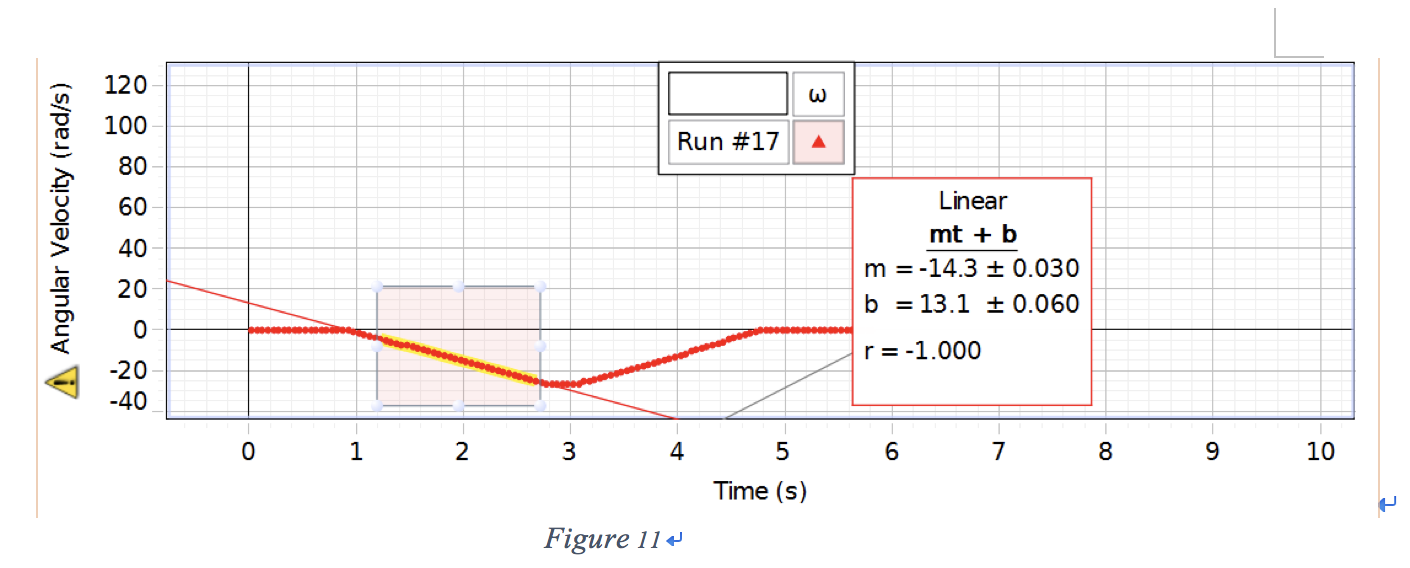
\includegraphics[width=15cm]{f_4_6}
\caption{The best-fit line for \emph{angular velocity} versus \emph{time} graph}
\label{linear regression}
\end{figure}
From the graph we observe that the \emph{angular acceleration} $\alpha$ is obtained:
\[
\alpha=14.3\pm0.030\text{rad/$s^2$}.
\]
\subsection{Data and Error Analysis}
\subsubsection{Method 1:}
By applying Eq.(\ref{Eq._6}) to Eq.(\ref{Eq._10}) together with the data from Table(\ref{Data collected manually for each type of disk}), we could compute the \emph{theoretical} momentum inertia about its center of mass for each type of disk:
\begin{center}
\begin{tabular}{|p{3cm}<{\centering}|p{6cm}<{\centering}|}
\hline
Pendulum Type &  Theoretical $I_{\text{cm}}$\\
						&	($\text{kg}\cdot\text{m}^2$)\\
						\hline

Disk 			&		$7.1224\times10^{-5}\pm1.8\times10^{-6}$\\
\hline
Disk with Hole 			&		$1.0049\times10^{-4}\pm1.2\times10^{-6}$\\
\hline
Thin Ring 			&		$4.0514\times10^{-5}\pm1.1\times10^{-6}$	\\
\hline
Thick Ring 			&		$6.2545\times10^{-5}\pm1.5\times10^{-6}$		\\
\hline
Irregular Shape 	&	$/$			\\
\hline
\end{tabular}
\fcaption{Theoretical inertia for each type of disk}\label{Theoretical inertia for each type of disk}
\end{center}
\begin{itemize}
\item\textbf{Error Explanation: }
For disk, the error is given by:
\begin{align*}
\delta I_{cm}&=\sqrt{\left(\frac{\partial I_{cm}}{\partial M}\right)^2(\delta M)^2+\left(\frac{\partial I_{cm}}{\partial R}\right)^2(\delta R)^2}\\
&=\sqrt{\left(\frac{1}{2}R^2\right)^2(\delta M)^2+\left(MR\right)^2(\delta R)^2}\\
&=\sqrt{\left(\frac{1}{2}(0.04m)^2\right)^2(5\times10^{-5}\text{kg})^2+\left(0.089\cdot0.04\right)^2(5\times10^{-4}m)^2}\\
&=1.8\times10^{-6}\text{kg}\cdot\text{m}^2.
\end{align*}
Following the similar idea, we could derive the error for the inertia of the remaining kinds of disks.
\end{itemize}
\subsubsection{Method 2:}
Using Eq.(\ref{Method_1}) together with the \emph{average period} data from Table(\ref{Average Period for each type of disk: Data collected from Capstone}) and the data for the \emph{mass} of the disk from Table(\ref{Data collected manually for each type of disk}), we could compute the \emph{momentum of inertia} indirectly:
\begin{center}
\begin{tabular}{|p{3cm}<{\centering}|p{6cm}<{\centering}|}
\hline
Pendulum Type &  Derived $I_{\text{cm}}$\\
						&	($\text{kg}\cdot\text{m}^2$) $(\pm3\times10^{-6}\text{kg}\cdot\text{m}^2)$\\
						\hline

Disk 			&		$7.4160\times10^{-5}$\\
\hline
Disk with Hole 			&		$9.9961\times10^{-5}$\\
\hline
Thin Ring 			&		$3.7237\times10^{-5}$	\\
\hline
Thick Ring 			&		$6.3912\times10^{-5}$		\\
\hline
Irregular Shape 	&	$5.8912\times10^{-5}$			\\
\hline
\end{tabular}
\fcaption{Theoretical inertia for each type of disk}\label{Theoretical inertia for each type of disk}
\end{center}
\begin{itemize}
\item\textbf{Error Explanation:}
The error of momentum of inertia is given by:
\begin{align*}
\delta I_{cm}&=
\sqrt{\left(\frac{\partial I_{cm}}{\partial T}\right)^2(\delta T)^2+\left(\frac{\partial I_{cm}}{\partial M}\right)^2(\delta M)^2+\left(\frac{\partial I_{cm}}{\partial L_c}\right)^2(\delta L_c)^2}\\
&=
\sqrt{\left(\frac{TMgL_c}{2\pi^2}\right)^2(\delta T)^2
+
\left(\frac{T^2gL_c}{4\pi^2}-L_c^2\right)^2(\delta M)^2
+
\left(\frac{T^2Mg}{4\pi^2}-2ML_c\right)^2(\delta L_c)^2}\\
\end{align*}
Following this way we derive the error for the momentum of inertia. The process of plugging in data into this large formula is skipped.
\end{itemize}
\subsubsection{Method 3:}
And we could use another way to compute the momentum inertia for irregular shape disk. During this part, the inertia is derived as:
\begin{align*}
I&=\frac{rm(g-r\alpha)}{\alpha}\\
&=\frac{0.014\text{m}\times0.01\text{kg}\times(9.8\text{m}/s^2-0.014\text{m}\times14.3\text{rad/}s^2)}{14.3\text{rad/}s^2}\\
&=6.2791\times10^{-5}\text{kg}\cdot\text{m}^2.
\end{align*}
The error for the inertia of irregular shape is
\begin{align*}
\delta I&=\sqrt{\left(\frac{\partial I}{\partial\alpha}\right)^2(\delta \alpha)^2}\\
&=\left|
-\frac{rmg}{\alpha^2}-r^2m
\right|\delta \alpha\\
&=\left(
\frac{0.014\text{m}\times0.01\text{kg}\times9.8\text{m}/s^2}{(14.3\text{rad/}s^2))^2}+(0.014\text{m})^2\cdot(0.01\text{kg})
\right)(0.030\text{rad/}s^2))^2)\\
&=3.6\times10^{-6}\text{kg}\cdot\text{m}^2.
\end{align*}
Hence the inertia of the irregular shape disk is given by:
\[
I=6.2791\times10^{-5}\pm3.6\times10^{-6}\text{kg}\cdot\text{m}^2.
\]
\subsubsection{Difference}
We could use \textbf{Method 1} and \textbf{Method 2} to compute the momentum inertia of the first four types of disk in Figure(\ref{Different kinds of disks}). And we compare these two different results. The difference for two calculated inertia is given by:
\[
\text{Difference } = \frac{\text{Theoretical inertia} - \text{Derived inertia}}{\text{Derived inertia}}\times100\%
\]
After plugging in specific data, we obtain the difference for these four difference kinds of disks:
\begin{center}
\begin{tabular}{|p{3cm}<{\centering}|p{3cm}<{\centering}|}
\hline
Pendulum Type &  Difference\\
						\hline

Disk 			&		$-3.96\%$\\
\hline
Disk with Hole 			&		$0.53\%$\\
\hline
Thin Ring 			&		$8.80\%$	\\
\hline
Thick Ring 			&		$6.17\%$		\\
\hline
\end{tabular}
\fcaption{Theoretical inertia for each type of disk}\label{Theoretical inertia for each type of disk}
\end{center}
And we could use \textbf{Method 2} and \textbf{Method 3} to compute the momentum inertia of the irregular shape disk. The difference for two calculated inertia is given by:
\begin{align*}
\text{Difference} &= \frac{5.8912\times10^{-5}\text{kg}\cdot\text{m}^2 - 6.2791\times10^{-5}\text{kg}\cdot\text{m}^2}{6.2791\times10^{-5}\text{kg}\cdot\text{m}^2}\times100\%\\
&=-6.18\%
\end{align*}
\section{Conclusion}
\begin{itemize}
\item
In experiment 1, theoretically when the distance between the pivot and the center of mass is $8.1$cm, the period of oscillation is minimized. And experimentally we found when the distance is $8.0$cm, the period of oscillation is minimized. The difference between the theoretical value and the measured value for the length is $1.23\%$, which is very small. Hence we conclude the validity of this experiment.\\
Moreover, according to Eq.(\ref{Eq._4}), a heavier or lighter bar with the same dimensions should have the same value for the length that gives minimum period of oscillation. Mass is not a factor in the calculation of the length for minimum period.
\item
In experiment 2, as we can see in Table(\ref{Theoretical inertia for each type of disk}), the difference between the inertia calculated by period and inertia calculated by dimensions is relatively small. For irregular shape, the difference between the inertia calculated by period and inertia calculated by acceleration is also relatively small. Hence we confirm the validity of our experiment.
\end{itemize}












\end{document}